\section{Problem A: Pathfinding in 2D Games}

All deliverables in the form of code are included aside the report.

\subsection*{Subproblem A.1: Grids with Obstacles}

The following figures show the solution path calculated by the A* implementation,
with the $\text{OPEN}$ and $\text{CLOSED}$ sets visualized as respectively blue
and red dots.

\begin{figure}[h!]
  \centering
    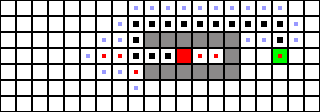
\includegraphics[width=0.5\textwidth]{img/board-1-1-astar}
    \caption{Board 1.1}
\end{figure}

\begin{figure}[h!]
  \centering
    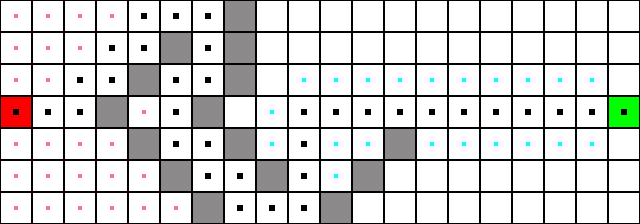
\includegraphics[width=0.5\textwidth]{img/board-1-2-astar}
    \caption{Board 1.2}
\end{figure}

\begin{figure}[h!]
  \centering
    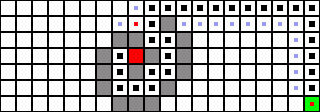
\includegraphics[width=0.5\textwidth]{img/board-1-3-astar}
    \caption{Board 1.3}
\end{figure}

\begin{figure}[h!]
  \centering
    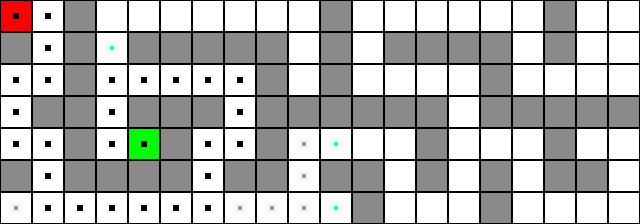
\includegraphics[width=0.5\textwidth]{img/board-1-4-astar}
    \caption{Board 1.4}
\end{figure}

\newpage


\subsection*{Subproblem A.2: Grids with different cell costs}

For this subproblem, we modified our implementation to be able to parse weighted
boards as well as correctly handling cost calculation of weighted nodes.
Again, the visualizations include the $\text{OPEN}$ and $\text{CLOSED}$ sets.

\begin{figure}[h!]
  \centering
    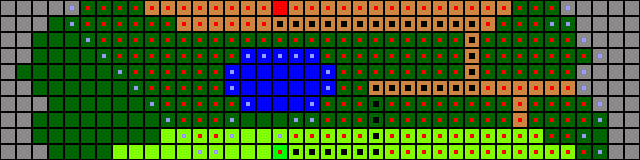
\includegraphics[width=0.8\textwidth]{img/board-2-1-astar}
    \caption{Board 2.1}
\end{figure}

\begin{figure}[h!]
  \centering
    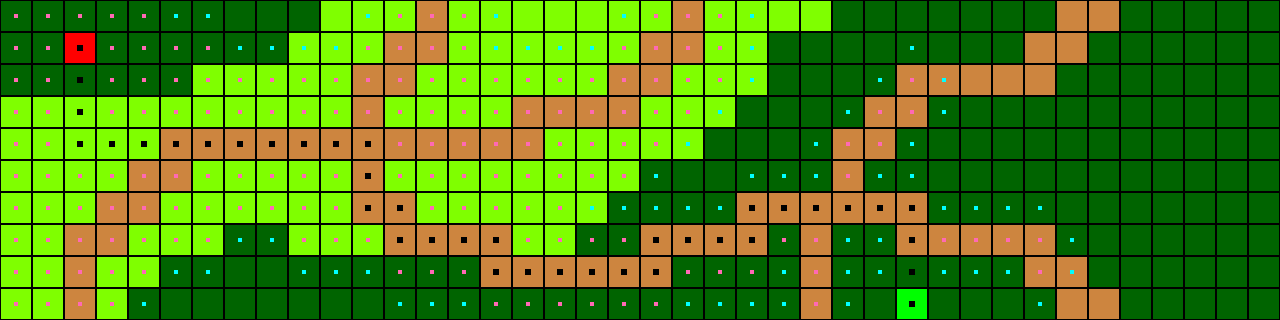
\includegraphics[width=0.8\textwidth]{img/board-2-2-astar}
    \caption{Board 2.2}
\end{figure}

\begin{figure}[h!]
  \centering
    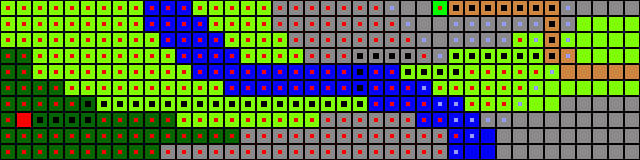
\includegraphics[width=0.8\textwidth]{img/board-2-3-astar}
    \caption{Board 2.3}
\end{figure}

\begin{figure}[h!]
  \centering
    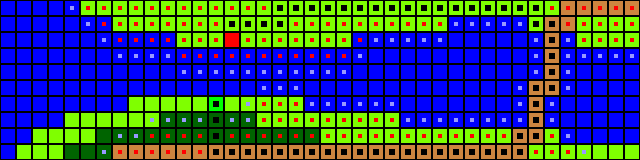
\includegraphics[width=0.8\textwidth]{img/board-2-4-astar}
    \caption{Board 2.4}
\end{figure}

\newpage

\subsection*{Comparison with BFS and Dijkstra's Algorithm}


